\subsection{Unexpected Surprises: The Flip Side of Noise Blankers!}

\begin{tcolorbox}[colback=gray!10, colframe=black, title=E4E09`]
What undesirable effect can occur when using a noise blanker? 

\begin{enumerate}[label=\Alph*.]
    \item Received audio in the speech range might have an echo effect
    \item The audio frequency bandwidth of the received signal might be compressed
    \item \textbf{Strong signals may be distorted and appear to cause spurious emissions}
    \item FM signals can no longer be demodulated
\end{enumerate} \end{tcolorbox}

\subsubsection{Related Concepts}

Noise blankers are used in radio communication to suppress unwanted noise, often caused by electrical interference. However, they can introduce their own set of problems, primarily concerning signal distortion. 

\subsubsection{Understanding the Correct Answer}

The correct answer, option C, refers to the phenomenon where strong incoming signals, when processed by a noise blanker, may become distorted. This distortion can lead to spurious emissions, which are unintended signals emitted by a device that can cause interference with other communications.

When a noise blanker is engaged, it operates by checking the incoming signal levels and suppressing sudden pulses of interference. However, if the incoming signal is too strong, the blanker may inadvertently distort the desired signal. 

\subsubsection{Signal Distortion Explained}

To explain this distortion, consider the following steps:

1. \textbf{Incoming Signal Strength}: A strong incoming signal that exceeds a certain threshold.
2. \textbf{Blanking Function Activation}: The noise blanker activates to suppress noise.
3. \textbf{Distortion Trigger}: The blanking function inadvertently alters the shape and characteristics of the desired signal.
4. \textbf{Spurious Emissions}: This alteration leads to unintended frequencies being generated, leading to spurious emissions.

\subsubsection{Visual Representation}

A basic diagram illustrating the incoming signal, the effect of the noise blanker, and the resulting distortion can be developed using TikZ. Below is a simplified representation:

\begin{tcolorbox}
\begin{center}
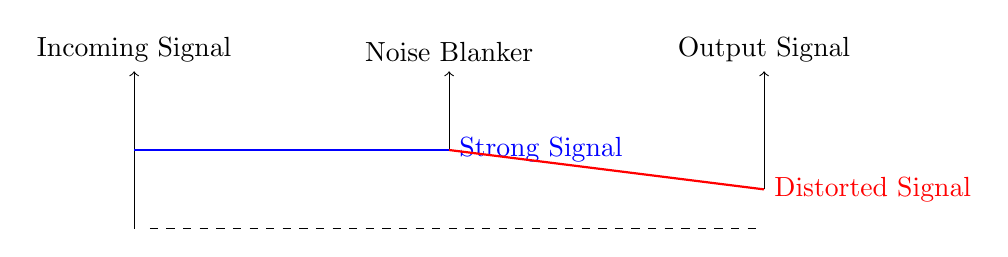
\begin{tikzpicture}
    % Incoming signal
    \draw[->] (0,0) -- (0,2) node[above] {Incoming Signal};
    \draw[thick, blue] (0,1) -- (4,1) node[right] {Strong Signal} ;
    
    % Noise Blanker effect
    \draw[->] (4,1) -- (4,2) node[above] {Noise Blanker};
    \draw[thick, red] (4,1) -- (8,0.5) node[right] {Distorted Signal};
    
    % Output signal
    \draw[->] (8,0.5) -- (8,2) node[above] {Output Signal};
    \draw[dashed] (0.2,0) -- (8,0); % baseline
\end{tikzpicture}
\end{center}
\end{tcolorbox}
